% !TeX root = Stageportfolio.tex



\begin{landscape}
	
	\subsubsection{Les 6-8}
	\begin{tabularx}{1.56\textwidth}{|p{0.55\textwidth}|X|}\hline
		\textbf{Administratieve gegevens}\newline\newline
		Kevin Truyaert\newline\newline
		Universiteit\newline
		Handelsingenieur, 2de fase\newline
		\underline{ECTS-fiche}: De inhoud is terug te vinden op de ECTS fiche: \href{https://onderwijsaanbod.kuleuven.be/syllabi/n/D0W55AN.htm}{https://onderwijsaanbod.kuleuven.be/syllabi/n /D0W55AN.htm} \newline
		\underline{Lesonderwerp}: `DC netwerken met weerstanden' & \textbf{Doelstellingen}\newline\vspace{0.5cm}
		\underline{Punt op de ECTS-fiche}
		\vspace{-0.5cm}\newline  - DC netwerken, wetten van Kirchhoff, elektrische meettoestellen \newline - toepassing: elektrische veiligheid en elektrische huisinstallatie \newline
		\underline{Lesdoelen}\newline
		\vspace{-0.5cm}
		\begin{enumerate}[itemsep=0.08\baselineskip]
			\item De studenten kennen de wetten van Kirchhoff.
			\item De studenten kunnen de wetten van Kirchhoff conceptueel uitleggen.
			\item De studenten kunnen de wetten van Kirchhoff opstellen voor een open netwerk met bronnen en weerstanden.
			\item De studenten kunnen de wetten van Kirchhoff opstellen voor een gesloten netwerk met bronnen en weerstanden.
			\item De studenten kunnen interpreteren dat een voltmeter gebruiken zorgt voor een wijziging in de spanningsval over een component. 
		    \item De studenten kunnen in groep over de oefening discussiëren en samen oplossingsgericht werken.
		\end{enumerate} \\\hline
	\multicolumn{2}{c}{ }\\
	\multicolumn{2}{c}{ }\\
	\multicolumn{2}{c}{ }\\
	\multicolumn{2}{c}{ }\\
	\multicolumn{2}{c}{ }\\
	\multicolumn{2}{c}{ }\\
	\multicolumn{2}{c}{ }\\
	\multicolumn{2}{c}{ }\\
	\multicolumn{2}{c}{ }\\
	\multicolumn{2}{c}{ }\\
	\end{tabularx}


	\begin{tabularx}{1.56\textwidth}{|p{0.55\textwidth}|X|}
		\hline
		\multirow{2}{0.55\textwidth}{\textbf{Beginsituatie}\newline De studenten hebben de theorie rond de wetten van Kirchhoff drie weken voor de oefenzitting gezien. Hierdoor zullen ze al tijd gehad hebben om de theorie te bekijken. Rond deze tijd hebben de studenten echter meerdere deadlines voor andere vakken en een examen Frans. Hierdoor plaats ik geen voorbereidende oefening online, maar vraag ik hen om enkel de wetten van Kirchhoff nog eens goed te bekijken. \newline\newline Er zijn 28 studenten die deze sessie volgen, maar vorige sessie waren slechts 18 studenten aanwezig. \newline\newline Het lokaal kan 30 studenten plaatsen. Ik splits de groep in zeven tafels van vier personen. Er is een dubbel krijtbord ter beschikking en de mogelijkheid tot projectie. Wanneer er geprojecteerd wordt, hangt het projectiescherm grotendeels over beide borden.  }& \textbf{Acties}\newline  - Net zoals tijdens de eerste lessenreeks, wil ik de studenten in \GreenHighlight{groepjes van vier studenten}{5cm} aan de slag zetten. Als examenvraag stel ik namelijk een oefening op rond de wetten van Kirchhoff, die aansluit bij wat ze deze en volgende les te zien krijgen. Ik vind het van essentieel belang dat ze de wetten van Kirchhoff niet allen goed en veel kunnen oefenen, maar dat ze die ook conceptueel begrijpen. Bij de eerste lessenreeks merkte ik op dat ik op deze manier gerichtere feedback aan de studenten kon geven. Ik ervoer ook dat ze gemotiveerd waren om per twee `beter' te doen dan hun overburen, terwijl ze toch steevast elkaar hielpen wanneer de andere vast zaten. Ik wil hier opnieuw een steunende rol spelen tijdens hun leer- en ervaringsproces.  \newline\newline
		
		- Bij het begin van de les overloop ik samen met de studenten de wetten van Kirchhoff. Zij reiken mij de twee wetten aan, die ik op het bord neerschrijf. Verder noteer ik ook samen met hen een stappenplan om dit soort oefeningen op te lossen. Dit laat ik op het bord staan. Zo kunnen de studenten steeds makkelijk teruggrijpen naar de theorie. \newline\newline
		- Ik werk niet met projectie, maar noteer alles op het bord, omdat het projectiescherm voor zo goed als beide borden hangt. Hierdoor houd ik een tempo aan waarop de studenten makkelijker kunnen volgen, doordat ik alles zelf ook neerschrijf.  
		
		\\ \cline{2-2}
		  & \textbf{Bronnen}\begin{itemize}
		  	\item Dudal, D., Temmerman, E., Truyaert, K., Heymans, S. (2019). Slides conceptuele natuurkunde
		  	\item Dudal, D., Temmerman, E., Truyaert, K., Heymans, S. (2019). Oefeningenbundel conceptuele natuurkunde
		  	\item Giancoli, D. C. (2008). Physics for scientists and engineers. Pearson Education International.
		  \end{itemize}\\ \hline
	\end{tabularx}


\newpage

\begin{tabularx}{1.56\textwidth}{|p{1.5cm}|p{6cm}|X|p{3cm}|}
	\hline
	\textbf{Nr. lesdoel } & \textbf{Inhoud (timing)}  & \textbf{Organisatie } & \textbf{Media } \\ \hline
	1\newline 2 &\underline{Herhaling theorie (20 minuten)}\newline
	De theorie rond de wetten van Kirchhoff worden door de studenten aangereikt. Zij interpreteren ook wat de vergelijkingen voorstellen en delen dit met hun medestudenten. Hierna bouw ik samen met de studenten een stappenplan op om dit soort oefeningen aan te pakken. We bespreken ook nog kort even welke voorwaarden voldaan moeten zijn om een stroom te hebben (gesloten kring, geen condensatoren). 
	&  \underline{Onderwijsleergesprek}\newline 
	Ik start deze les met aan de studenten te vragen om mij de twee wetten van Kirchhoff uit te leggen. Ik noteer de wiskunde vertaling hiervan op bord. Ik probeer verschillende studenten aan het woord te laten.\newline Hierna stel ik samen met de studenten een stappenplan op om DC schakelingen te kunnen interpreteren. Ik vermoed dat de studenten dit zich niet meer goed zullen herinneren vanuit de theorieles. Daardoor zal ik zelf eerst een hint per stap geven of de stap(pen) zelf op het bord zetten, waarna ik telkens nog eens een student aan het woord laat om deze stap uit te leggen in eigen woorden. Hierna schets ik een kleine kring op het bord waar we dit klassikaal op toepassen.\newline
	Ik focus mij ook hier weer op het correct interpreteren van beide vergelijkingen. Dit is goed mogelijk door een vergelijking te maken waarbij de stroom een rij mensen of een rij auto's is en een spanningsverschil een helling. De eerste wet wordt dan  dat je bij ieder kruispunt slecht één richting kan kiezen waardoor het totaal aantal inkomende mensen/auto's hetzelfde moet zijn aan het totaal vertrekkende auto's. De tweede wet van Kirchhoff stelt voor dat je in iedere kring op hetzelfde niveau moet terugkomen: als je een kring doorlopen hebt, dan ben je terug op dezelfde hoogte.
	\newline 
	Hierna noteer ik de oefeningen op bord die gemaakt kunnen worden. Dit zijn oefeningen 66, 65, 69 en 71 in die volgorde. Ik verwacht dat de alle oefeningen door iedereen gemaakt kunnen worden.\newline Ik zal de nadruk tijdens deze les vooral leggen op het zelfstandig inoefenen van dit soort oefeningen. Na het stappenplan op het bord genoteerd te hebben en met een minimaal voorbeeld gelinkt te hebben, heb ik uit ervaring van de voorbije jaren gemerkt dat de studenten er geen meerwaarde aan hebben om nog eerst een extra oefening te maken. Daarom laat ik hen meteen aan de slag gaan met de oefeningenreeks.
	& Krijtbord (Bordschema in bijlage)
	\\ \hline
\end{tabularx}




\begin{tabularx}{1.56\textwidth}{|p{1.5cm}|p{6cm}|X|p{4cm}|}
	\hline
	\textbf{Nr. lesdoel } & \textbf{Inhoud (timing)}  & \textbf{Organisatie } & \textbf{Media } \\ \hline
	3\newline 4\newline 6 &\underline{Oefening 66 (30 minuten)}\newline
	Ik laat de studenten eerst zelf aan de slag gaan om per twee/vier aan deze oefening te beginnen. Ondanks dat ze in de theorieles al enkele DC netwerken overlopen hebben en nu een stappenplan nog eens expliciet opgesteld hebben, zullen ze nog niet volledig begrijpen hoe dit soort oefeningen aan te pakken. De voorbije jaren moest ik telkens expliciet minstens één oefening helemaal klassikaal begeleiden, nadat ze er zelf aan gewerkt hebben. Hier zal ik ook nu voor zorgen.
	&  \underline{Check-in duo / check-in quatro}\newline
	De eerste 15 minuten wil ik de studenten laten in hun groep per twee of per vier aan de slag laten gaan. Het is de eerste maal dat ze zelfstandig dit soort oefening maken, dus ik verwacht een trage start. Ondanks het stappenplan, zullen de studenten enkele vragen hebben. Daarom geef ik duidelijk mee dat ik de eerste vijf minuten niet zal rondlopen. Deze tijd gebruik ik om de schakeling op het nog vrije bord te tekenen.\newline
	Daarna loop ik rond en observeer ik de studenten, stel ik vragen of beantwoord die. Na een kwartier verwacht ik dat er weinig oplossingen en veel vragen uit de bus gekomen zijn. Daarom bespreek ik deze oefening nog eens klassikaal, door het stappenplan met hen te overlopen. Ik lees nog eens duidelijk de stap en vraag aan de studenten wat ik moet doen.\newline
	Ik verwacht dat de studenten niet allemaal alle inzichten hebben, waardoor ik dit stappenplan klassikaal `bevraag'. Zo zullen niet alle studenten er bij stil gestaan hebben dat er geen stroom doorheen de open takken stromen, waardoor ze een vergelijking minder nodig hebben. Ik verwacht dan ook dat de studenten hier vragen over zullen hebben tijdens het oplossen van de opdracht. Hiervoor reken ik in totaal ook een kwartier uit.
	& Bord\newline Oefeningenbundel + cursuspapier
	\\ \hline
\end{tabularx}


\begin{tabularx}{1.56\textwidth}{|p{1.5cm}|p{6cm}|X|p{4cm}|}
	\hline
	\textbf{Nr. lesdoel } & \textbf{Inhoud (timing)}  & \textbf{Organisatie } & \textbf{Media } \\ \hline
	4\newline 5\newline 6 &\underline{Oefening 65 (25 minuten)}\newline
	Deze oefening toont aan dat wanneer je de spanningsval wil meten over een verbruiker, de interne weerstand heel groot moet zijn om de reële situatie op te meten. Want wanneer je iets meet, verander je steeds de uitkomst. Bij deze oefening heeft de voltmeter geen hoge interne weerstand, waardoor het spanningsverschil gemeten over beide componenten lager ligt dan het spanningsverschil van de bron.
	& 	\underline{Check-in duo / check-in quatro}\newline
	De oefening zelf zal deze keer beter gaan, in vergelijking met de vorige. De studenten hebben nu het stappenplan op drie verschillende manieren ervaren: bij een minimaal voorbeeld, zelf geprobeerd en klassikaal. Ik verwacht deze keer de grootste problemen bij het verwerken van de voltmeter in de schakeling. Verder zie ik hen de oefening goed oplossen.\newline
	Aan de studenten die vlotter weg zijn met deze oefening, zal ik extra vragen hoe het komt dat de som van de twee opgemeten potentiaalverschillen niet die van de bron is. Dit zou fysisch moeten kloppen, aangezien je anders geen behoud van energie zou hebben. Deze vraag wil ik vooral conceptueel behandelen: doordat je een weerstand in parallel plaatst, verandert de equivalente weerstand en verandert het systeem. Om dit zoveel mogelijk te beperken, zorg je dat je voltmeter een hoge interne weerstand heeft. Deze vraag stel ik op het eind van dit lesonderdeel klassikaal aan de overige studenten, omdat ik het concept `Meten is weten' wil verduidelijken naar `Meten is veranderen en interpreteren'.
	& Oefeningenbundel + cursuspapier
	\\ \hline
\end{tabularx}






\begin{tabularx}{1.56\textwidth}{|p{1.5cm}|p{6cm}|X|p{4cm}|}
	\hline
	\textbf{Nr. lesdoel } & \textbf{Inhoud (timing)}  & \textbf{Organisatie } & \textbf{Media } \\ \hline
		&\underline{Pauze}\newline
	
	
	&    De studenten krijgen 15 minuten pauze en mogen het lokaal verlaten. Op deze manier kunnen ze het laatste uur weer met volle aandacht werken. 
	Wanneer de eerste studenten het lokaal terug binnen sijpelen, sla ik een praatje met hen, waarbij ik niet over de leerstof begin. 
	& 
	\\ \hline
\end{tabularx}


\begin{tabularx}{1.56\textwidth}{|p{1.5cm}|p{6cm}|X|p{4cm}|}
	\hline
	\textbf{Nr. lesdoel } & \textbf{Inhoud (timing)}  & \textbf{Organisatie } & \textbf{Media } \\ \hline
	4\newline 6&\underline{Oefeningen  69 en 71 (55 minuten)}\newline
	Deze oefeningen behandelen iets complexere schakelingen met weerstanden. De studenten leren tijdens deze lesfase verder de wetten van Kirchhoff inoefenen op iet complexere systemen.
 &  \underline{Check-in duo / check-in quatro}\newline
 De studenten lossen deze complexere oefeningen in overleg met elkaar op. Ik loop rond om vragen te beantwoorden en om in te pikken op hun reeds gevonden oplossing, zowel wanneer die correct of foutief blijkt te zijn. Ik wil hier vooral de nadruk blijven leggen op het conceptuele van de fysische concepten, naast het correct oplossen van de vraag. Hoe de studenten de richtingen van hun stroom en potentiaalverschillen definiëren maakt enkel uit over de bronnen (indien er meerdere aanwezig zijn), maar niet bij verbruikers (dan komen ze gewoon negatief uit). 
	& Oefeningenbundel + cursuspapier
	\\ \hline
\end{tabularx}



\begin{tabularx}{1.56\textwidth}{|p{1.5cm}|p{6cm}|X|p{4cm}|}
	\hline
	\textbf{Nr. lesdoel } & \textbf{Inhoud (timing)}  & \textbf{Organisatie } & \textbf{Media } \\ \hline
	&\underline{Afsluiten (5 minuten)}\newline 
	&  \underline{Afsluiten (5 minuten)}\newline
	Ik herhaal nog even kort wat er van de studenten verwacht werd tijdens deze les en wat ze bijgeleerd hebben. Ik zeg ook dat volgende oefenzitting de laatste is en dat ze, indien gewenst, dan vragen kunnen stellen.
	& 
	\\ \hline
\end{tabularx}


	
	
	
	
	
	
\end{landscape}



\subsection*{Bijlage 3.1: bordschema theorie}
\begin{center}
	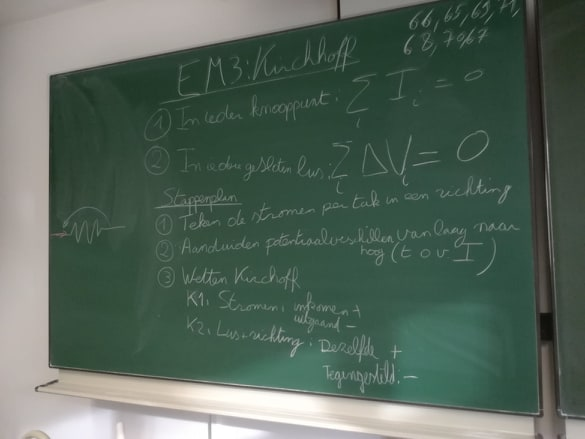
\includegraphics[width=0.9\textwidth]{Bord3}
\end{center}
\newpage
\subsection*{Bijlage 3.2: opgeloste oefeningen}




